Emando B.V. is een jong bedrijf dat maatwerksoftware maakt. Momenteel ontwikkelt Emando voor de \acf{KNSB} een nieuw licentie-aankoop- en -beheersysteem, een nieuw wedstrijdadministratiesysteem en een nieuwe schaatstijdendatabase. Naar aanleiding van eerder contact met de \ac{KNSB} over toegang tot de schaatstijdendatabase zijn wij in telefonisch contact gekomen met Johan Stokking van Emando. Tijdens het oriënterende gesprek bleek dat zowel wij als Emando er geïnteresseerd in waren dat wij ons Bachelor Eindproject bij Emando zouden uitvoeren, onder begeleiding van de heer Stokking.

\section{Opdrachtsamenvatting}
In de weken voorafgaand aan het Bachelor Eindproject is in samenspraak met Emando de opdrachtomschrijving gemaakt. Bij het brainstormen zijn de minimale eisen en de mogelijke extra functies bedacht:

\begin{quotation}
\itshape
Het ontwerpen en ontwikkelen van een systeem voor het weergeven en analyseren van (live) recreatieve en trainingsdata in de context van baansporten (bijvoorbeeld schaatsen en baanwielrennen). Dit systeem zal realtime gegevens van de baan, maar ook opgeslagen gegevens uit het verleden, inzichtelijk maken voor sporters, coaches en eventuele toeschouwers (volgers). Daarnaast zal er de mogelijkheid zijn om een sociale component en een competitie element toe te voegen, en een mogelijkheid om aggregatie op data uit te voeren.

Het systeem ondersteunt het sporten: sporters hoeven hun training niet te onderbreken, doordat audio-cue's en sport-specifieke schermen geïmplementeerd worden. De sociale component bestaat uit het volgen van vrienden (mede-sporters) en het delen van resultaten. Het competitie element zal een virtuele competitie tussen vrienden omvatten.

Technisch gezien zal er een scheiding gemaakt worden tussen de diverse toepassingen (clients) en de API. De API biedt toegang tot realtime data en de diverse modulaire (sport-specifieke) aggregaties, waarbij de mogelijkheid bestaat voor bijvoorbeeld coaches om te abonneren op meerdere sporters. De API zal gekoppeld worden op bestaande systemen die data van transponders ontsluiten.
\end{quotation}

Om richting te geven aan het toekomstige applicatie, is de opdrachtomschrijving ambitieus opgesteld. We hebben vanaf het begin de instelling gehad om eerst een minimale versie te maken die werkt, om vervolgens de eerste versie uit te bouwen tot een volwaardige applicatie.

Zoals te lezen is in de opdracht zal er zowel een mobiele applicatie als een back-end systeem ontwikkeld worden. In sectie \ref{sec:programma-van-eisen} worden de elementen uit de opdrachtomschrijving uitgesplitst en omgezet in functionaliteiten met de bijbehorende prioriteit.

\section{Doelgroep en Gebruikers}

\newcommand{\doelgroep}{}
\label{sec:doelgroep}

\subsection{Schaatsers}
De voornaamste doelgroep van onze applicatie zijn de recreatieve en amateur schaatsers. Zij moeten met behulp van onze applicatie meer inzicht krijgen in hun prestaties en trainingen. 
Om er voor te zorgen dat deze groep gebruikers onze applicatie verkiest boven de reeds bestaande (minder uitgebreide) systemen, dienen zij snel en gemakkelijk met de applicatie aan de slag te kunnen gaan.
Bij een té ingewikkeld systeem zullen zij afhaken en de overstap naar onze applicatie wellicht niet willen maken.
Omdat zij de belangrijkste doelgroep zijn van de applicatie, is het belangrijk dat zij gemotiveerd worden om de applicatie te blijven gebruiken en hen tevens motiveren om ook anderen aan te sporen dit te doen.
Met behulp van sociale componenten zoals trainingsgroepen, het volgen van andere schaatsers en leaderboards kan onze applicatie hen hierin stimuleren.
\subsection{Coaches}
Als tweede doelgroep zijn er de coaches van de schaatsers. Dit zijn mensen die de schaatsers begeleiden bij hun trainingen en wedstrijden. Zij beschikken zelf niet altijd over een transponder, omdat niet iedere coach zelf schaatst.
Zij willen graag snel en gemakkelijk inzicht in de data van de schaatsers die zij coachen. Het moet voor hen dus gemakkelijk zijn om snel tussen schaatsers te kunnen switchen en deze prestaties zowel onderling als per training gemakkelijk te kunnen vergelijken.
\subsection{Overige gebruikers}
Tot slot is er de groep gebruikers die zelf geen deel uitmaakt van de schaatswereld. Zij zijn geen schaatsers of coaches en zijn met name geïnteresseerd in de mogelijkheden van de applicatie en het volgen van kennissen of bekende schaatsersn.
Ook zij moeten in staat zijn om de applicatie gebruiken, weliswaar in mindere mate.

\section{Reeds bestaande vergelijkbare systemen}

\newcommand{\vergelijkbaresystemen}{}
\label{sec:vergelijkbare-systemen}

Er bestaan al enkele oplossingen die functionaliteit bieden die vergelijkbaar is met die van de applicatie die wij gaan bouwen. Strava (figuur~\ref{fig:strava}) en RunKeeper (figuur~\ref{fig:runkeeper}) maken gebruik van GPS om onder andere hardlopers en wielrenners van realtime informatie te voorzien. \mylaps Practice (figuur~\ref{fig:mylapspractice}) is een website waar je na je training je prestaties kan terugkijken. Er bestaat ook een iPhone App voor \mylaps Practice (figuur~\ref{fig:mylapspractice-app}). Coach Watch (figuur~\ref{fig:coachwatch}) is een iPad applicatie waarmee coaches hun teams kunnen volgen.

\begin{figure}[ht]
\centering
\subfigure[Strava]{
    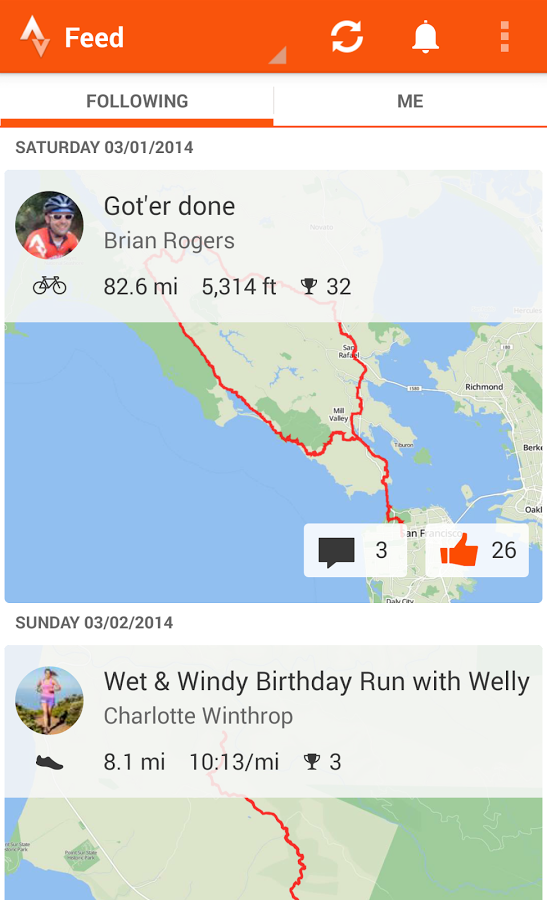
\includegraphics[height=5cm]{style/images/Strava}
    \label{fig:strava}
}
\subfigure[RunKeeper]{
    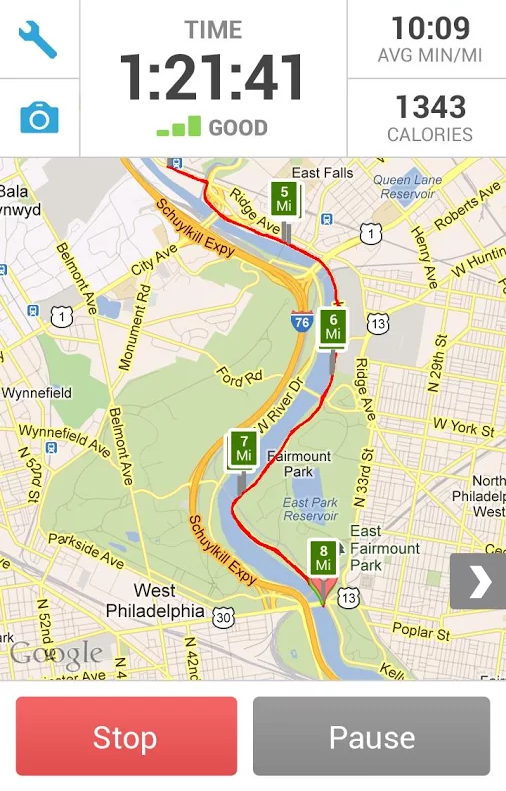
\includegraphics[height=5cm]{style/images/RunKeeper}
    \label{fig:runkeeper}
}
\subfigure[Coach Watch]{
    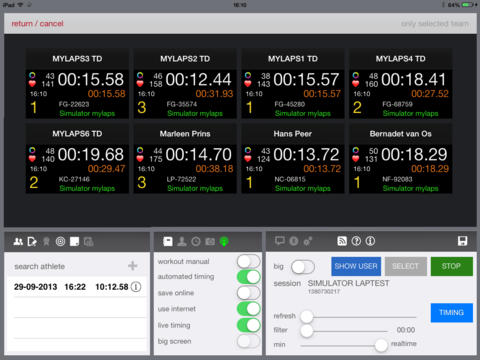
\includegraphics[height=5cm]{style/images/CoachWatch}
    \label{fig:coachwatch}
}

\subfigure[\mylaps Practice]{
    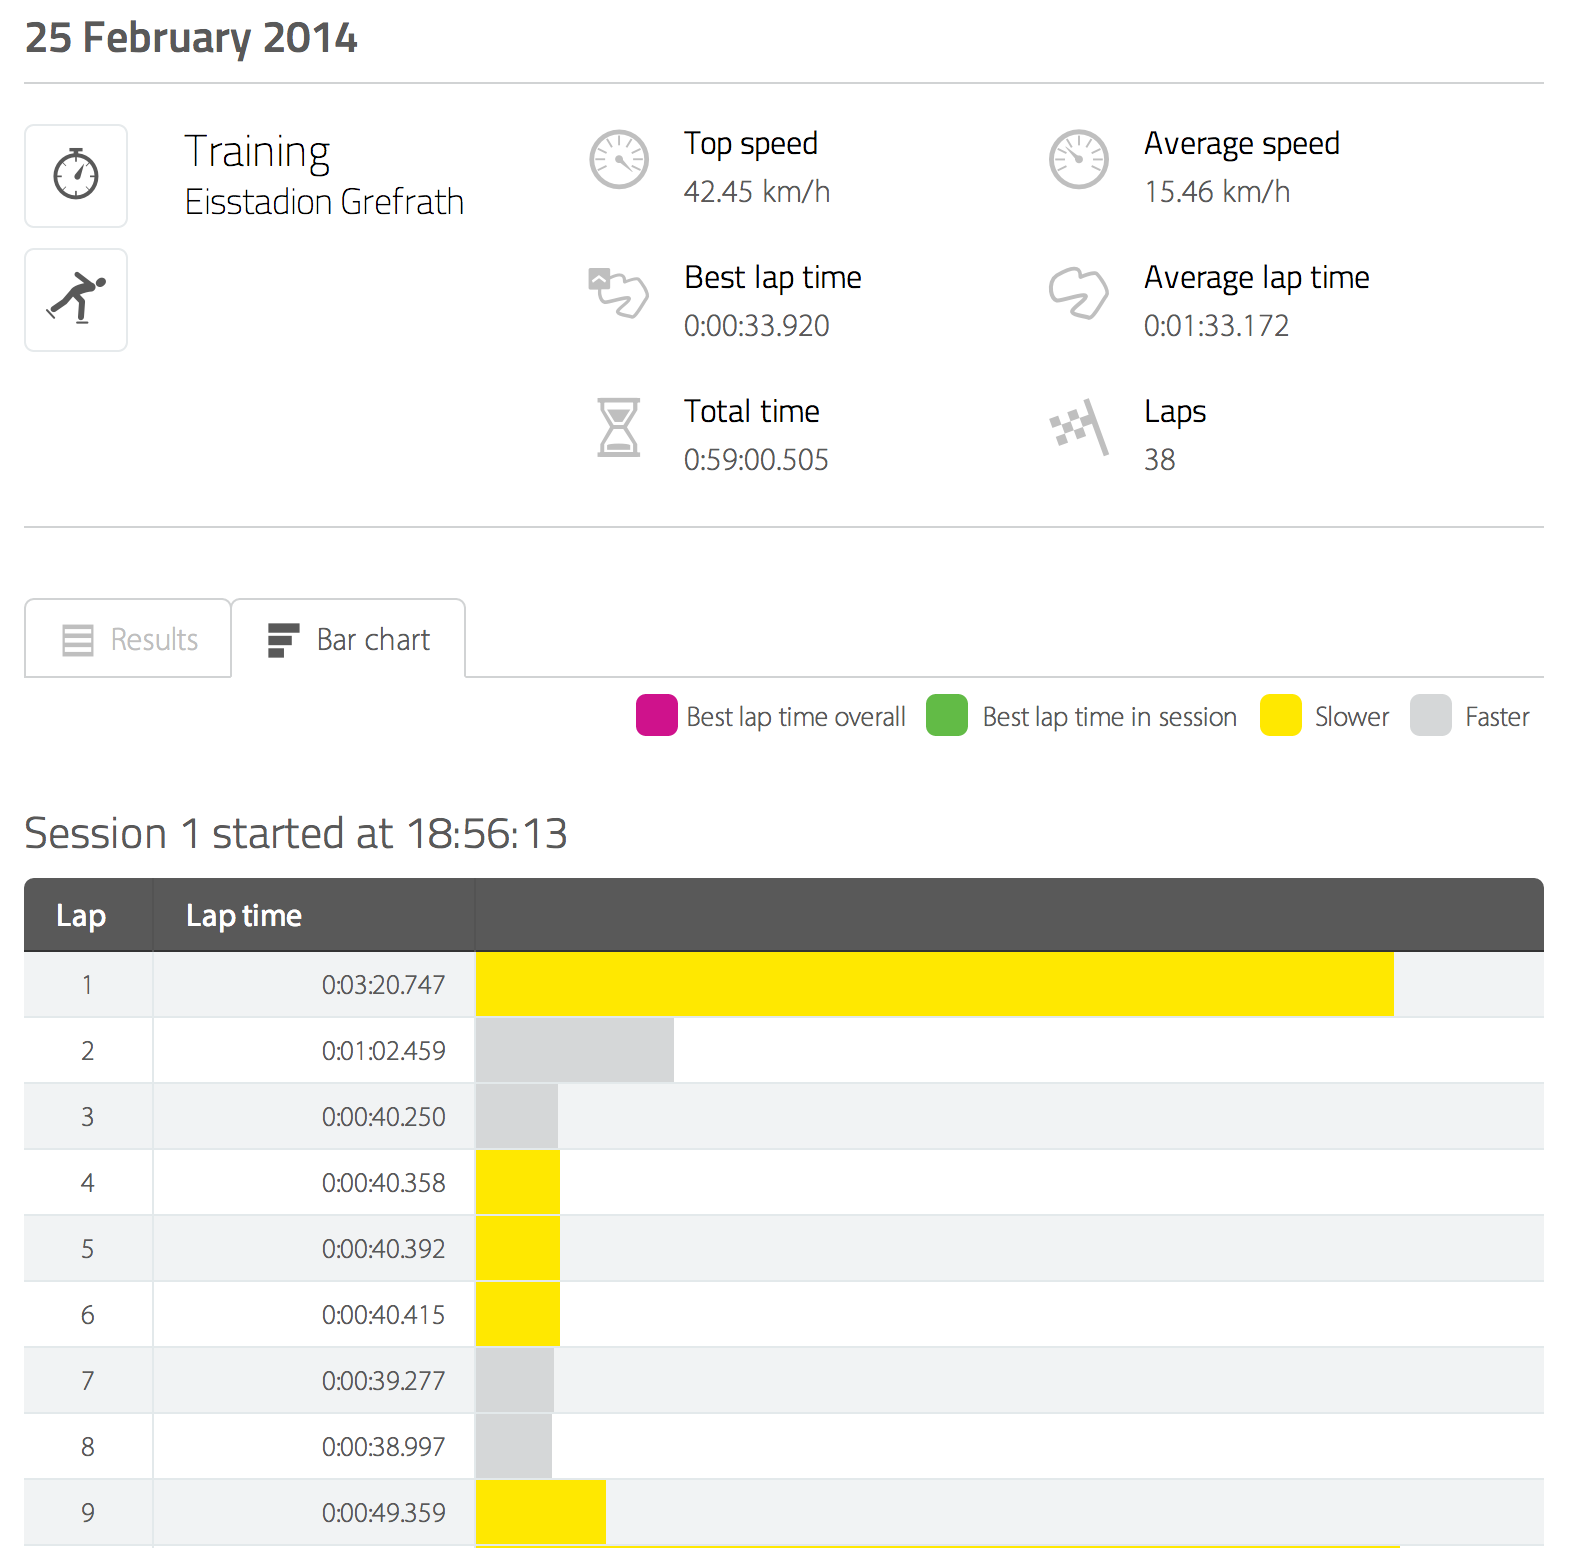
\includegraphics[height=7cm]{style/images/MyLapsPractice}
    \label{fig:mylapspractice}
}
\subfigure[\mylaps Practice App]{
    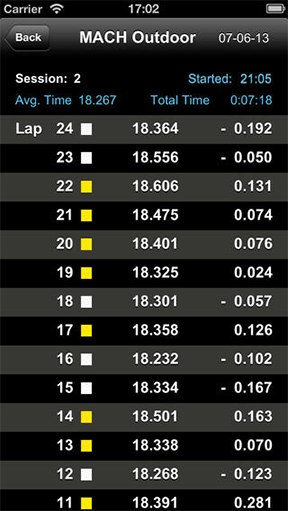
\includegraphics[height=7cm]{style/images/MyLapsPractice-App}
    \label{fig:mylapspractice-app}
}

\caption{Soortgelijke oplossingen}
\label{fig:soortgelijke-oplossingen}
\end{figure}

Strava en RunKeeper zijn voor baansporten, zoals bijvoorbeeld schaatsen, niet goed bruikbaar, aangezien GPS op de banen slecht presteert, waardoor de informatie niet nauwkeurig genoeg is. \mylaps Practice en Coach Watch maken wel gebruik van de detectielussen in de banen. De \mylaps Practice website kan alleen gebruikt worden voor het achteraf bekijken van sportprestaties en deze de applicatie is vooral gericht op motorsporten. CoachWatch is een (vrij dure) applicatie die vooral gericht is op coaches en dus minder geschikt voor trainingen of voor amateurschaatsers.

Emando ziet de mogelijkheid om een applicatie te bieden die gebruikmaakt van de detectielussen in de banen, die live gegevens kan tonen op een smartphone en die ook nog eens goedkoop of gratis is. Onze applicatie richt zich dus op het invullen van de stukken die missen in de bestaande oplossingen.
    
    % systemen in ontwikkeling bij Emando
\section{Programma van eisen} % MoSCoW shizzle

\newcommand{\programmavaneisen}{}
\label{sec:programma-van-eisen}

Traditioneel gezien wordt bij software ontwikkeling het MoSCoW model gebruikt. Het MoSCoW model onderscheid functionaliteiten op basis van prioriteiten. De verschillende niveau's zijn must-, should-, could- en won't-haves. De vertaling van deze niveau's spreekt voor zich.

Wij gebruiken het in combinatie met SCRUM veel gebruikte \acf{mvp} model. Hierbij wordt gedefinieerd wat het product minimaal moet kunnen om bruikbaar te zijn. In die zin komt onze \ac{mvp} dus overeen met de must-haves uit het MoSCoW model. Eventuele tegenslagen mogen er niet toe lijden dat het \ac{mvp} niet gemaakt wordt, daarom is de planning om het \ac{mvp} al in de 4e week af te hebben. Gebruikers kunnen op dat moment met de applicatie spelen en de kern-functionaliteit beoordelen.

Het \ac{mvp} biedt op zich zelf nog niet alle features die zowel wij als de opdrachtgever graag geïmplementeerd zouden willen zien. Het eindproduct zal over enkele bijzondere functies moeten beschikken, de zogenaamde `killer-features' om het product populair te maken. Deze features zijn in die zin dus vergelijkbaar met de should-haves uit het MoSCoW model.

Na het \ac{mvp} en de features die het verschil maken zijn er ook nog een aantal features die niet noodzakelijk zijn en geen groot verschil zouden maken. Deze features zijn te vergelijken met could-haves uit het MoSCoW model. We zullen zeker niet alle could-haves implementeren, en wellicht komen enkele should-features ook niet aan bod. Wellicht volgt uit een user study dat de door ons bedachte could-haves door users erg gewenste features zijn. In overleg met onze begeleiders kunnen we besluiten deze features te implementeren. Bovendien bieden de could-haves een goede leidraad bij toekomstige ontwikkeling na afloop van ons project.

\subsubsection{Must-haves (\ac{mvp})}

\begin{itemize} \parskip0pt \parsep0pt
    \item Bruikbaar als applicatie op smartphone(s)
    \item Architectuur is sport-agnostisch
    \item De sport-specifieke weergave van tijden is voor schaatsbanen geïmplementeerd
    \item Mogelijkheid om een account aan te maken
    \item Real-time transponder doorkomsten tonen van geselecteerde sporters
    \item Historische doorkomsten van een persoon, gegroepeerd per dag of training
    \item De voor bovenstaande features ontwikkelde API, moet het mogelijk maken om de API uit te breiden en de applicatie aan te passen.
\end{itemize}

\subsubsection{Should-haves}

\begin{itemize} \parskip0pt \parsep0pt
    \item Mogelijkheid om account te koppelen aan Facebook
    \begin{itemize}
        \item Mogelijkheid om prestaties en records te delen op Facebook
    \end{itemize}
    \item Audio-cues geven aan sporter over doorkomsten van een geselecteerde transponder
    \item Leaderboards tonen met sporters gerangschikt naar prestaties en disciplines (virtuele competitie), zoals:
    \begin{itemize}
        \item rondetijd (actuele/gemiddelde/snelste)
        \item snelheid (gemiddelde/snelste)
        \item cumulatieve afstand (per seizoen/week/training)
        \item rust/intensief-ratio (hoeveelheid rondjes, ratio)
        \item achievements-punten (verbeter jezelf 10\%, voor 7 uur op de baan, 2 trainingen per week)
    \end{itemize}
    
    \item Groepen-functionaliteit \begin{itemize}
        \item Mogelijkheid om een lege groep te maken
        \item Mogelijkheid om sporters uit te nodigen voor een groep
        \item Mogelijkheid om op uitnodiging in een groep te gaan
        \item Mogelijkheid om uit een groep te gaan
    \end{itemize}

    \item Zowel leaderboards als real-time doorkomst-schermen kunnen worden gefilterd op groep of baan
     
    \item Privacy instellingen bieden aan gebruikers
    \begin{itemize}
        \item Mogelijkheid om een account publiekelijk of anoniem te laten indexeren
        \item Mogelijkheid om eigen data te delen met anderen
    \end{itemize}

\end{itemize}

\subsubsection{Could-haves}

\begin{itemize} \parskip0pt \parsep0pt
    \item Suggesties krijgen om met soortgelijke schaatsers te gaan schaatsen
    \item Training kunnen exporteren naar RunKeeper\footnote{Fitness logboek platform, \url{http://www.runkeeper.com}}
\end{itemize}

\subsubsection{Won't-haves}

Het door Emando ontwikkelde systeem Vantage zal de huidige systemen voor wedstrijduitslagen vervangen. Koppelingen op het huidige systeem zouden dus snel niet meer werken en het nieuwe systeem is niet af tijdens ons project.
\begin{itemize} \parskip0pt \parsep0pt
    \item Wedstrijdloting en uitslagen bekijken
    \item Persoonlijke records tonen
\end{itemize}
